
\chapter{Implementation}
\label{chap:implementation}

In this chapter are described implementation details of the project.
Sections in this chapters explains individual problems and their solutions.
The text accompanies actual source code snippets and diagrams for better explanation.


Initially the project was named as \emph{Malsys} which stands for \emph{Mark's \lsystems} and this name preserved till now.
Thus root namespace is called \emph{Malsys}.


\section{Solution structure}

The solution is divided into 6 projects: \lsystem processing library (Malsys), web user interface (Malsys.Web), abstract syntax tree (Malsys.Ast), syntax parser (Malsys.Parsing), common functionality (Malsys.Common) and project with tests (Malsys.Tests).

The main reason why solution do not contain lower amount of projects is because syntax parser is written in F\# which is also language from .NET family but it is not possible to compile F\# and C\# into single DLL.
Abstract syntax tree (AST) is separated from parser because AST will be compiled by compilers written in C\# and it is desirable to have AST data structures written in C\#.
It is also more comfortable to design AST classes in C\# because F\# is functional language and syntax of classes definition is quite complex.
Common functionality is separated into single project because it will be needed in all projects and solution can not have circular dependencies of projects.
Web project is separated from main project intentionally to allow usage of \lsystem processing library independently.
And finally test project is separated to be possible to test all projects independently.
Dependencies of projects in solution are shown in the \autoref{fig:solutionDependencies}.
The \emph{Malsys.Tests} project has dependencies to all other projects.

\begin{figure}[h]
	\centering
	\begin{tikzpicture}[->,>=latex,shorten >=2pt]
		\node (c) [block] {Malsys.Common};
		\node (m) [block, below=of c] {Malsys};
		\node (a) [block, right=of m] {Malsys.Ast};
		\node (p) [blockx, right=of a] {Malsys.Parsing};
		\node (w) [block, left=of m] {Malsys.Web};
		\node (t) [block, below=2cm of m, xshift=2cm] {Malsys.Tests};
		\node (cSharp) [block, minimum width=1em, minimum height=1em, above=1cm of p] {C\#};
		\node (fSharp) [blockx, minimum width=1em, minimum height=1em, right=0.5cm of cSharp] {F\#};
		
		\draw (a) -- (c);
		
		\draw (p) to[bend right=10] (c);
		\draw (p) -- (a);
		
		\draw (m) -- (c);
		\draw (m) to[bend right=30] (p);
		\draw (m) -- (a);
		
		\draw (w) to[bend left=20] (c);
		\draw (w) -- (m);
		\draw (w) to[bend right=30] (a);
		
		\draw [shorten >=3.4cm] (t) -- (c);
		\draw [shorten >=1.2cm] (t) -- (a);
		\draw [shorten >=2cm] (t) -- (w.south);
		\draw [shorten >=1.2cm] (t) -- (m);
		\draw [shorten >=2cm] (t) -- (p.south);
	\end{tikzpicture}
	\caption{Dependencies of projects in solution}
	\label{fig:solutionDependencies}
\end{figure}


\section{Input parsing}
\label{sec:parsingImplementaion}

Input parsing is in the \emph{Malsys.parsing} project and it have two phases, lexing and parsing.
Lexing phase uses the lexer to convert input source codes to stream of \emph{tokens} (basic blocks of input) from which the parser parses the abstract syntax tree (AST).
The lexer is generated by the \emph{FsLex} tool [\ref{sec:FSharpPowerPack}].
Rules for the \emph{FsLex} are written using regular expressions and F\# code.
\autoref{code:fsl} shows an example of lexer definition of the \emph{FsLex} tool.
Full definition is in the file \emph{Lexer.fsl} in the \emph{Malsys.parsing} project.

\begin{Fsharp}[label=code:fsl,caption={Example of definition file for \emph{FsLex}}]
let whitespace = [' ' '\t']
let digit = '\Nd'  // unicode group for digits
// uppercase, lowercase, titlecase, modifier, other, number (letter)
let letter = '\Lu' | '\Ll' | '\Lt' | '\Lm' | '\Lo' | '\Nl'
// punctuation (connector), nonspacing, spacing, other (format)
let specialChar = '\Pc' | '\Mn' | '\Mc' | '\Cf'
let idFirstChar = letter | '_'
let idChar = letter | specialChar | digit | ['\'']
let id = idFirstChar idChar*

rule tokenize args = parse
    | whitespace { tokenize args lexbuf }  // ignore whitespaces
    | id { match keywords.TryFind(lexeme lexbuf) with
        | Some(token) -> token  // keyword
        | None -> ID(lexeme lexbuf) }  // identifier
    | digit+ { parseInt args lexbuf ConstantFormat.Float }
    ...
\end{Fsharp}

After lexing comes parsing.
Parser is generated by \emph{FsYacc} tool [\ref{sec:FSharpPowerPack}] from definition file (\emph{Parser.fsy} in the \emph{Malsys.parsing} project).
Parser is written to parse input to the abstract syntax tree (defined in \emph{Malsys.ast}.
All data structures in AST are immutable\footnote{Immutable data structures can not be changed after creation} which helps to robustness of the project.
It is impossible to change value of some node of AST by mistake.
\autoref{code:fsl} shows an example of parser definition.

\begin{Fsharp}[label=code:fsy,caption={Example of definition file for \emph{FsYacc}}]
// constant definition
ConstDef:
    | LET Id EQUALS Expression SEMI
      { new ConstantDefinition($2, $4, getPos parseState) }
 // function definition     
FunDef:
    | FUN Id OptParamsParens FunBody
      { new FunctionDefinition($2, $3, $4, getPos parseState) }
FunBody:
    | LBRACE FunStatementsList RBRACE
      { new ImmutableListPos<IFunctionStatement>(
      		$2, getPos parseState) }
FunStatementsList:
    |
      { new ResizeArray<IFunctionStatement>() }
    | FunStatementsList FunStatement
      { $1.Add($2); $1 }
FunStatement:
    | ConstDef
      { $1 :> IFunctionStatement }
    | RETURN Expression SEMI
      { $2 :> IFunctionStatement }
// identifier
Id:
    | ID
      { new Identifier($1, getPos parseState) }
\end{Fsharp}

Both \emph{FsLex} and \emph{FsYacc} tools are automatically run on build of the project in Visual studio.


\section{Compilation and evaluation}

Compilation of the abstract syntax tree is done by set of compilers defined in the \emph{Compilers} namespace in the \emph{Malsys} project.
There are defined specialized compilers for each part of the AST.
Compilers uses each other to compile the AST.
For example \emph{Input compiler} uses \emph{\lsystem compiler} which uses \emph{Constant definition compiler} etc.
\autoref{fig:compilers} shows the hierarchy of compilers.
To keep the figure clear arrows to \emph{Expression compiler} was shortened (every compiler uses the \emph{Expression compiler}).

\begin{figure}[h]
	\centering
	\begin{tikzpicture}[->,>=latex,shorten >=2pt]
		\node (in) [block] {Input comp.};
		\node (fd) [block, below=of in] {Function def. comp.};
		\node (ls) [block, left=of fd] {Lsystem comp.};
		\node (cd) [block, right=of fd] {Constant def. comp.};
		\node (ps) [block, left=of in] {Process stat. comp.};
		\node (pa) [block, below=of fd] {Parameters comp.};
		\node (rr) [block, below=of pa] {Rewrite rule comp.};
		\node (sy) [block, below=2cm of ls] {Symbols comp.};
		\node (ex) [block, below right=3cm of fd] {Expression comp.};
		
		
		\draw (in) -- (cd);
		\draw (in) -- (fd);
		\draw (in) -- (ls);
		\draw (in) -- (ps);
		
		\draw (fd) -- (cd);
		\draw (fd) -- (pa);		
		
		\draw (ls) to [bend left=21] (cd);
		\draw (ls) -- (fd);
		\draw (ls) -- (pa);
		\draw (ls) to [bend right=10] (rr);
		\draw (ls) -- (sy);
		
		\draw (ps) -- (ls);
		
		\draw (rr) to [bend right=10] (cd);
				
		\draw (cd) -- (ex);
		\draw (rr) -- (ex);
		\draw [shorten <=1cm] (pa) -- (ex);
		\draw [shorten <=3cm] (fd) -- (ex);
		\draw [shorten <=5.5cm] (sy) -- (ex);
		\draw [shorten <=6.5cm] (ls) -- (ex);
		\draw [shorten <=5cm] (in) -- (ex);
		\draw [shorten <=8.5cm] (ps.south) -- (ex);
	\end{tikzpicture}
	\caption{Hierarchy of compilers}
	\label{fig:compilers}
\end{figure}


Compilers are not bound to the graph statically.
All compilers implements general interface and they requires other compilers through the interfaces (\autoref{code:compIfaces}).
Each compiler takes all dependent compilers as parameters of the constructor.

\begin{Csharp}[label=code:compIfaces,caption={General interface for compilers, interface for the constant definition compiler and its implementation}]
// general interface for simplifying definition of compilers interfaces
public interface ICompiler<TSource, TResult> {
	TResult Compile(TSource obj, IMessageLogger logger);
}

// constant definition compiler compiles Ast.ConstantDefinition to ConstantDefinition
public interface IConstantDefinitionCompiler
	: ICompiler<Ast.ConstantDefinition, ConstantDefinition> {}

// concrete implementation of constant definition compiler interface	
public class ConstantDefCompiler : IConstantDefinitionCompiler {
		// constructor
		public ConstantDefCompiler(@IExpressionCompiler expressionCompiler@) { ... }
		// compile method
		public ConstantDefinition Compile(Ast.ConstantDefinition constDefAst,
			IMessageLogger logger) { ... }
}
\end{Csharp}

Inversion of control (IOC) \nomenclature{IOC}{inversion of control} container is used to instantiate all compilers [\ref{sec:autofac}].
All types of compilers are registered to the IOC container then it is possible to resolve instances and all dependencies are resolved by the container.
This approach also bring great simplicity and extensibility.
\autoref{code:compCont} shows implementation of the compilers container and its possible usage.

\begin{Csharp}[label=code:compCont,caption={General interface for compilers and interface for the expression compiler}]
public class CompilersContainer : ICompilersContainer {
	protected IContainer container;  // the IOC container	

	public CompilersContainer() {
		var builder = new ContainerBuilder();
		builder.@RegisterType<InputCompiler>().As<IInputCompiler>()@.SingleInstance();
		...  // registration of all other compilers
		container = builder.Build();
	}

	public T Resolve<T>() {
		return container.Resolve<T>();
	}
}

// possible usage
var inputContainer = new CompilersContainer().@Resolve<IInputCompiler>()@;
\end{Csharp}

The result of compilation is a semantic tree.
The semantic tree is as well as AST immutable.

All compilation errors are logged sing the \emph{IMessageLogger} class.
No exceptions are thrown which helps performance and error recovery (compile can continue even after non fatal errors). 

\subsubsection*{Evaluation}

Evaluation of semantic tree is implemented in the same way as the compilation.
There is set of evaluators and IOC container links them together.



\section{Components members}
\label{sec:compImplementaion}

Component is .NET class.
All components must implement the \emph{IComponent} interface (\autoref{code:IComponent}) and they must have parameter-less constructor.

\begin{Csharp}[label=code:IComponent,caption={Interface of the \emph{ProcessManager} class}]
public interface IComponent {
	IMessageLogger Logger { set; }
	void Initialize(ProcessContext context);
	void Cleanup();
}
\end{Csharp}

According to \autoref{sec:components} components can have settable properties, settable symbol properties, gettable properties, connection properties, callable functions and interpretation methods.
All of them must be marked with special attribute to be possible to distinguish from other class properties and methods.
The access name of all members is the same as their real name.
However the \emph{AccessName} attribute can be used to change it.

\subsubsection{Component lifetime}
\label{sec:componentLifetime}

The \emph{IComponent} have two basic methods, the \emph{Initialize} and \emph{Cleanup}.
Following list shows the order of individual operation during creation of the component graph.

\begin{itemize*}
	\item instantiation (using required parameter-less constructor),
	\item set of \emph{Logger} property \lsystem:
	\item for each processed \lsystem:
	\begin{itemize*}
		\item reset (cleanup) with \emph{Cleanup} method, it should be used for setting component to default state
		\item connecting other components (setting connection properties)
		\item setting of settable (symbol) properties
		\item initialization with \emph{Initialize} method
		\item processing of \lsystem
	\end{itemize*}
	\item cleanup with \emph{Cleanup} method.
\end{itemize*}



\subsubsection{Settable properties}

Settable properties (and settable symbol properties) are properties of the component class marked with the \emph{UserSettable} (\emph{UserSettableSybols}) attribute.
Properties must have public setter (getter is not required).
Settable properties must have type assignable to the \emph{IValue} which covers two base types, numbers (\emph{Constant} type) and arrays (\emph{ValuesArray} type).
Settable symbol properties must have type \emph{ImmutableList<Symbol<IValue>{}>}.

By default all settable (symbol) properties are optional which means that their value may not be set.
By setting the \emph{IsMandatory} property of the \emph{UserSettable} (\emph{UserSettableSybols}) attribute to true is the property marked as mandatory and error will be thrown if no value is set to it.

Setter of settable (symbol) properties can throw \emph{InvalidUserValueException} if supplied value is invalid.
The text of the exception will be shown as an error to the user.



\subsubsection{Gettable properties}

Similarly as settable properties, gettable properties are properties of the component class marked with the \emph{UserGettable} attribute.
Properties must have public getter (setter is not required) and they must have type assignable to the \emph{IValue}.

By default values of gettable properties can be get after the initialization of the component.
In that time all the \lsystem in already evaluated thus they can not be used in \lsystem statements.
However it is possible to set the \emph{IsGettableBeforeInitialiation} property of the \emph{UserGettable} attribute to allow getting of property before initialization and to use its value in \lsystem statement.


\subsubsection{Connection properties}

Connection properties are for connecting of other components.
They are properties of the component class marked with the \emph{UserConnectable} attribute.
Properties must have public setter (getter is not required) and their type must be assignable to the \emph{IComponent} type.

Connection of some component to connection properties is by default mandatory but it is possible to set the \emph{IsOptional} property of the \emph{UserConnectable} attribute to allow leaving property unconnected (\emph{null}).
By default only one component can be assigned (connected) to each connection property but this can be changed by the \emph{AllowMultiple} property of the \emph{UserConnectable} attribute.

Setter of connection property can throw \emph{InvalidConnectedComponentException} if supplied value of component is invalid.
The text of the exception will be shown as an error to the user.


\subsubsection{Callable functions}

Callable functions serves to allow calling of component methods in \lsystem code (in statements, rewrite rules etc.).
Callable functions are method of the component class marked with the \emph{UserCallableFunction} attribute.
The underlying method must have a parameter of type \emph{IValue[]} and they must return type assignable to the \emph{IValue}.

Similarly as gettable properties callable functions can be by default called after the initialization of the component but it is possible to set the \emph{IsCallableBeforeInitialiation} property of the \emph{UserCallableFunction} attribute to allow calling the function before initialization.


\subsubsection{Interpretation methods}

Interpretation methods are specialized methods used for interpretation of symbols.
Interpretation methods must be marked with the \emph{SymbolInterpretation} attribute, they must have a parameter of type \emph{ArgsStorage} and \emph{void} return type.


\subsection{Documentation of members}
\label{sec:componentDoc}

To simplify documentation of component and their members is is used standard XmlDoc with custom elements.
Documentation is loaded automatically if the XML file with documentation in included with DLL where the component is.

To document the component standard \emph{summary} tag is used.
The user readable name for the component can be written in the \emph{name} tag and for group to which component belongs is tag called \emph{group}.
Example of documentation of component is in \autoref{code:docExample}.

\begin{Csharp}[label=code:docExample,caption={Example of usage XmlDoc for documentation of component}]
/// <summary>
///	Provides symbol property called Axiom which serve as
/// initial string of symbols of L-system.
/// </summary>
/// <name>Axiom provider</name>
/// <group>Common</group>
public class AxiomProvider : SymbolProvider {
	...
}
\end{Csharp}



\subsubsection{Settable (symbol) properties}

Basic documentation is of settable property is loaded from \emph{summary} tag.
Expected valued description can be put into \emph{expected} and for the default value of settable property is \emph{default} tag.

For settable symbol property is loaded only \emph{summary} tag


\subsubsection{Gettable and connection properties}

Documentation for gettable  and connection properties is loaded from standard \emph{summary} tag.


\subsubsection{Callable functions and interpretation methods}

In addition to standard \emph{summary} tag for general documentation callable functions (and interpretation methods) can be documented with \emph{parameters} tag where on each line should be documentation for each parameter. 


\subsection{Example}

The example of implementation and documentation of component is in appendix \ref{chap:componentExample}.


\section{Input processing}
\label{sec:implInputProcessing}

Component graph creation is the core of the \lsystem processing library.
The class responsible for that is called \emph{ProcessManager} (\autoref{code:procMan}).

It uses the class \emph{ProcessConfigurationBuilder} for creation and configuration of the component graph.
For resolving component types the \emph{ProcessManager} uses the \emph{IComponentMetadataResolver}.
It works in similar way as IOC container but components do not have any dependencies.
Components are registered by user directly using the \emph{IComponentMetadataResolver} implementation or with helper class called \emph{MalsysLoader}.

\begin{Csharp}[label=code:procMan,caption={Interface of the \emph{ProcessManager} class}]
public class ProcessManager {

	public ProcessManager(ICompilersContainer compIoc,
		IEvaluatorsContainer evalIoc, @IComponentMetadataResolver compResolver@) {

	public InputBlockEvaled CompileAndEvaluateInput(string sourceCode,
		string sourcName, IMessageLogger logger) { ... }
		
	public void @ProcessInput@(InputBlockEvaled inBlock, IOutputProvider outProvider,
		IMessageLogger logger, TimeSpan timeout) { ... }
}
\end{Csharp}

\emph{ProcessManager} does following steps in the method \emph{ProcessInput}.
notice the similarities with compoennt lifetime (\autoref{sec:componentLifetime}).

For each process statement in the input do:
\begin{enumerate*}
	\item instantiate all components in the Process configuration (specified by process statement),
	\item \label{procStep2} save gettable properties and callable functions from components which can be get and called before initialization,
	\item for each \lsystem (specified by process statement) do:
	\begin{enumerate*}
		\item reset (clean) all components,
		\item connect components to graph (resetting may disconnect them),
		\item evaluate \lsystem, gettable properties and callable functions from step \ref{procStep2} can be used to evaluate \lsystem statements,
		\item evaluate additional \lsystem statements from process statement,
		\item set settable properties of all components (from evaluated \lsystem statements),
		\item save rest of gettable properties and callable functions from components,
		\item initialize all components,
		\item find starter component and start it,
	\end{enumerate*}
	\item reset (clean) all components.
\end{enumerate*}


\section{Immutable data structures as scoped storage}
\label{sec:immutableDs}

In many places in the \lsystem processing library there is need for temporary addition of constants to a collection.
As an example can be evaluation of function.
Parameters of the function are added as constants to the collection but this addition can overlay already defined constants.
After evaluation the collection should be in the same state as before (parameters and local variables must not remain).
This problem can be solved by complex mutable data structures or by defensive copying of collections which can lead to serious performance issues (there can be hundreds of defined constants).

\emph{Immutable data structures} offers clean solution to this problem.
Immutable data structure is data structure which can not be changed (muted) like \emph{string} in C\#.
They can not be changed thus there is no need for creation of defensive copies.
If method passes an immutable collection of defined constants to function evaluation method it can not be changed by it.

But if immutable data structures can not be changed how is possible to add new items to them?
It is not possible because they are immutable but it is possible to create new copy with added item.
Interestingly enough addition to immutable tree has the same asymptotic complexity as insertion to mutable tree.

Each node of immutable tree is immutable.
If we want to add new node we will find place in the tree where it should be.
Now we need to connect it to the parent but the parent is immutable so we will create new parent (copying value from old one) but with new connections.
Old children (if any) can be connected without re-creating them.
So we need to re-create only nodes on the path to the root so complexity is logarithmic ($log_2(n)$ new nodes).
Insertion to immutable tree is illustrated in \autoref{fig:immAdd}.

There is no need for implementation if immutable tree because he F\# contains it as class \emph{FSharpMap<TKey, TValue>} and the \emph{MapModule} class provides methods for the work with it.

This system ensures that global variables will be accessible and can be temporarily overlayed by more local definitions.
It is used in may places including evaluation of \lsystems (local constants and functions overlays local ones), evaluation of user-defined functions (parameters and local variables)
	and rewrite rules (parameters of symbols are mapped as local variables).
	


\tikzstyle{tree} = [draw, fill=blue!12, circle, minimum size=9mm]
\tikzstyle{treex} = [draw,thick, fill=red!12, circle, minimum size=9mm]

\begin{figure}[h!]
	\centering
	\subfloat[Original tree]{
	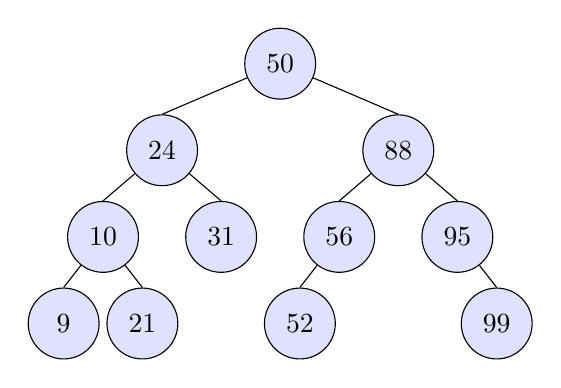
\begin{tikzpicture}[child anchor=north,>=latex,level/.style={sibling distance=30mm/#1},level distance=11mm]
		\node [tree] {50}
			child { node [tree] {24}
				child {node [tree] {10}
					child { node [tree] {9} }
					child { node [tree] {21} }
				}
				child { node  [tree] {31} }
			}
			child { node [tree] {88}
				child { node [tree] {56}
					child { node [tree] {52} }
					child [missing] {}
				}
				child { node [tree] {95}
					child [missing] {}
					child { node [tree] {99} }
				}
			}
			;
	\end{tikzpicture}
	} \hfill
	\subfloat[Tree with inserted node 71]{
	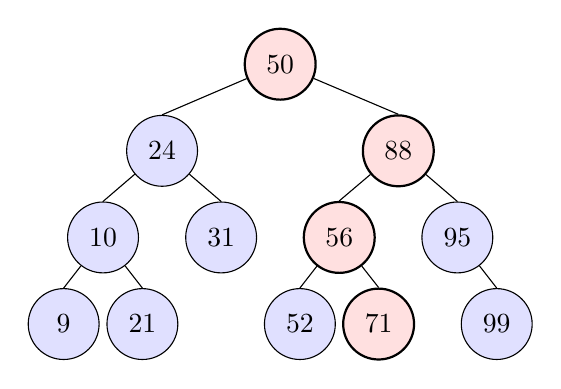
\begin{tikzpicture}[child anchor=north,>=latex,level/.style={sibling distance=30mm/#1},level distance=11mm]
		\node [treex] {50}
			child { node [tree] {24}
				child {node [tree] {10}
					child { node [tree] {9} }
					child { node [tree] {21} }
				}
				child { node  [tree] {31} }
			}
			child { node [treex] {88}
				child { node [treex] {56}
					child { node [tree] {52} }
					child { node [treex] {71} }
				}
				child { node [tree] {95}
					child [missing] {}
					child { node [tree] {99} }
				}
			}
			;
	\end{tikzpicture}
	}
	\caption{Example of addition to immutable tree, red nodes are newly created}
	\label{fig:immAdd}
\end{figure}


\section{Implemented components}

There are many implemented components in the \lsystem processing library.
In this section is described implementation details of some of them.


\subsection{Symbol rewriter}

The core of \lsystem processing is rewriteing of \lsystem symbols.
The \emph{SymbolRewriter} component is responsible just for that.
Its implementation supports all \lsystem types described in \autoref{sec:lsysTypes}.

The most complicated part is the context checking (in context rewrite rules) which satisfies rules about context checking defined in \autoref{sec:bracketedLsystems}.
It can not be implemented by naive approach which will search context symbols one by one because branches must be skipped and they can be very long.
\autoref{lsys:longContext} demonstrates an \lsystem where naive implementation will not be able to work well.
It uses symbol $S$ to generate random color index as its parameter.
Symbol $S$ is "linked" using context to every symbol $X$ which is rewritten to new branches with color index from base symbol $S$.
This causes that all lines in one iteration have same color but colors between iterations differs.
First five iterations with random seed set to 0 are in \autoref{fig:longContext}.

\begin{Lsystem}[label=lsys:longContext,caption={\lsystem }]
lsystem LongContext extends Branches {
	set symbols axiom = S(0) X;
	set symbols @contextIgnore = + - F@;
	set iterations = 5;
	set initialAngle = 90;	
	interpret F(c) as DrawForward(32, 2, c * #001100);
	interpret + as TurnLeft(20);
	interpret - as TurnLeft(-20);
	rewrite @{S(c)} X@ to [ + F(c) X ] - F(c) X;
	rewrite S to S(floor(random(0,16)));
}
process all with SvgRenderer;
\end{Lsystem}

\begin{figure}[h]
	\subfloat{\includegraphics[scale=0.9]{LongContext1}} \hfill
	\subfloat{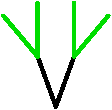
\includegraphics[scale=0.85]{LongContext2}} \hfill
	\subfloat{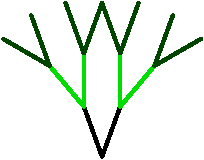
\includegraphics[scale=0.8]{LongContext3}} \hfill
	\subfloat{\includegraphics[scale=0.75]{LongContext4}} \hfill
	\subfloat{\includegraphics[scale=0.7]{LongContext5}}
	\caption{Result of \lsystem in \autoref{lsys:longContext}}
	\label{fig:longContext}
\end{figure}


In following list are strings of symbols of first five iterations of \lsystem in \autoref{lsys:longContext}.
Ignored symbols $+$, $-$ and $F$ are omitted.
Every symbol $X$ needs to search for the very first symbol to match the context correctly.
Now you can see why naive implementation can not be used.

\begin{enumerate*}
	\item S(0) X
	\item S(11) [ X ] X
	\item S(13) [ [ X ] X ] [ X ] X
	\item S(12) [ [ [ X ] X ] [ X ] X ] [ [ X ] X ] [ X ] X 
	\item S(8) [ [ [ [ X ] X ] [ X ] X ] [ [ X ] X ] [ X ] X ] [ [ [ X ] X ] [ X ] X ] [ [ X ] X ] [ X ] X 
\end{enumerate*}

The symbol rewrite component builds the tree from context which allows to skip branches quickly.
Tree nodes at the same level are interlinked to allow search for left and right context effectively.
The pointer to current symbol is updated after each processed symbol.
The tree is dynamically loaded as right context needs more symbols.
Three node is represented by class \emph{ContextListNode<T>}.
Class \emph{ContextListBuilder} helps to build the tree correctly symbol by symbol.

The search tries all possible ways to match the context but number of possible ways is relatively low.
\autoref{fig:contextChecking} shows an example of context search in tree built from fourth iteration of \lsystem in \autoref{lsys:longContext}.
Red path shows search for left context $S$ of symbol $X$ and green path shows search for right context $[X]$ of symbol $X$.
The search methods are located in the \emph{ContextChecker} class.

\tikzstyle{arr} = [draw, fill=blue!12, rectangle, minimum height=2em, minimum width=2em]
\tikzstyle{sym} = [draw, fill=red!12, rectangle, minimum height=2em, rounded corners=1mm]
\tikzstyle{arrow} = [draw=gray,<->,dashed,shorten >=2pt,shorten <=2pt]
\tikzstyle{path} = [draw=red,thick,->,shorten >=1pt]
\tikzstyle{path2} = [draw=green,thick,->,shorten >=1pt]

\begin{figure}[h!]
	\centering
	\begin{tikzpicture}[child anchor=north,>=latex,level/.style={sibling distance=33mm/#1}]
		\node [arr,] {root}
			child { node (a) [sym,draw=red, thick] {S(12)} }
			child { node (b) [arr] {[ ]}
				child { node (ba) [arr] {[ ]}
					child { node (baa) [arr] {[ ]}
						child { node (baaa) [sym] {X} }
					}
					child { node (bab) [sym] {X} }
				}
				child { node (bb) [arr] {[ ]}
					child { node (bba) [sym,draw=green, thick] {X} }
				}
				child { node (bc) [sym,draw=red, thick] {X} }
			}
			child { node (c) [arr] {[ ]}
				child { node (ca) [arr] {[ ]}
					child { node (caa) [sym] {X} }
				}
				child { node (cb) [sym] {X} }
			}
			child { node (d) [arr] {[ ]}
				child { node (da) [sym] {X} }
			}
			child { node(e) [sym] {X} }
			;
		\draw [arrow] (a) -- (b);
		\draw [arrow] (b) -- (c);
		\draw [arrow] (c) -- (d);
		\draw [arrow] (d) -- (e);
		
		\draw [arrow] (ba) -- (bb);
		\draw [arrow] (bb) -- (bc);
		
		\draw [arrow,dashed,shorten >=0,shorten <=0] (baa) -- (bab);
		
		\draw [arrow] (ca) -- (cb);
		
		\draw [draw=red,<-,thick,shorten <=2pt] (bc) -- +(0,-2cm);
		\draw [path] (bc) to[bend right=20] (bb);
		\draw [path] (bb) to[bend right=20] (ba);
		\draw [path,dashed] (ba) to[bend right=20] +(-1.2cm,0);
		\draw [path] (ba.north) ++(-0.2,0) to[bend left=20] (b);
		\draw [path] (b) to[bend right=20] (a);
		
		
		\draw [draw=green,<-,thick,shorten <=2pt] (bba) -- +(0,-2cm);
		\draw [path2] (bba) to[bend right=20] (bb);
		\draw [path2, dashed] (bb) to[bend right=20] (bc);
		\draw [path2] (bb) to[bend right=20] (b);
		\draw [path2] (b) to[bend left=20] (c);
		\draw [path2,dashed] (c) to[bend right=20] (ca);
		\draw [path2] (c) to[bend left=20] (d);
		\draw [path2] (d) to[bend right=20] (da);
		
		\node [area,fit=(d) (da),thick,green] {};
	\end{tikzpicture}
	\caption{Context search tree built from fourth iteration of \lsystem in \autoref{lsys:longContext}}
	\label{fig:contextChecking}
\end{figure}

As context matching method finds matching symbol it also maps its parameters to named variables.
Because context matching is done by back-track and mapped symbols can be invalid immutable data structures are used for saving mapped variables and roll-back to old values can be done with no cost (see \autoref{sec:immutableDs}).
Described algorithm is not optimal but it is sufficient for the most cases.
Production \lsystem have rarely context longer than one.

Context checking is tested by many unit tests in the \emph{Malsys.Tests} project which ensures correctness of implemented algorithm.


\subsection{Turtle graphics interpreter}

Turtle graphics interpreter implemented by class \emph{TurtleInterpreter} is universal interpreter for both 2D and 3D renderers.
It interprets symbols as turtle graphics in 3D but if 2D interpreter is connected it omits the Z coordinate.
This allows to use 3D commands in output rendered by 2D renderer which brings many advantages.
For example the \emph{Roll} (rotation by direction axis) by $180^{\circ}$ can be used for the inversion of turning directions in 2D.

Interpreter allows to use three basic rotations: pitch, yaw and roll.
Pitch operation turns up around right-hand vector, yaw turns left around up vector axis and roll operation rolls clock-wise around forward vector axis.
The up, right and forward vectors can be set using user settable properties allowing changes to coordinate system.

The rotation of turtle is represented as the \emph{Quaternion}.
This has many advantages because quaternions represent rotation around axis which is exactly what basic operations do.
In the contrast to representation of rotation by the rotation matrix the quaternion allows to is easy to pitch, yaw and roll by axes which are relative to current orientation.
Also the storage size of rotation represented by the quaternion is the smallest possible since quaternion is represented as four numbers.
Composition of two quaternion rotations is equal to multiplying them.
\autoref{code:yaw} shows code snippet of the \emph{Yaw} interpretation method of the \emph{TurtleInterpreter}.

%!!!!!!!!!!!!!!!Composition?

\begin{Csharp}[label=code:yaw,caption={Implementation of the \emph{Yaw} method of the \emph{TurtleInterpreter}}]
[SymbolInterpretation(1)]
public void Yaw(ArgsStorage args) {
	double angle = getArgumentAsDouble(args, 0);
	currState.Rotation *= new Quaternion(upVect, angle);
}
\end{Csharp}


The \emph{TurtleInterpreter} can simulate the tropism\footnote{A tropism is a biological phenomenon, indicating growth or turning movement of a biological organism, usually a plant, in response to an environmental stimulus.(\url{http://en.wikipedia.org/wiki/Tropism})}.
This is easily done by quaternions too because tropism is simulated as physical force which is applied to the line \cite[p.~58]{PL91} (\autoref{code:tropismImpl}).

\begin{Csharp}[label=code:tropismImpl,caption={Implementation of the tropism which is applied after each line}]
private void rotateByTropism(Vector3D moveVector) {
	Vector3D axis = Vector3D.CrossProduct(moveVector, tropismVect);
	double angle = axis.Length * tropismCoef;
	if (angle.EpsilonCompareTo(0) == 0) {
		return;
	}
	axis.Normalize();
	currState.Rotation = new Quaternion(axis, angle) * currState.Rotation;
}
\end{Csharp}


\section{Triangulation of 3D polygons}

Turtle graphics interpretation of \lsystems can generate polygons which are points in space that defines perimeter of an object.
In 2D tey form polygon which is easy to render even if its shape is complex (crossing edges etc.).
But in 3D the situation is much more complex because.
Lets call the object specified by points on its perimeter 3D polygon even if it is not 100\% technically correct.
3D polygon is specified by points on its perimeter but they does not say anything about the shape itself.
There is more possible interpretations even of basic polygons (example for 4 points is in \autoref{fig:3dSquare}).

\begin{figure}[h!]
	\hfill
	\subfloat{\includegraphics[width=0.3\linewidth]{3dSquare1}}
	\hfill
	\subfloat{\includegraphics[width=0.3\linewidth]{3dSquare2}}
	\hfill ~
	\caption{Ambiguous triangulation of four points}
	\label{fig:3dSquare}
\end{figure}

Because of the ambiguity in triangulation there can not exist ideal triangulation algorithm.
With this in the mind was written trianguler in \lsystem processing library.
It is possible to configure triangulation strategies.

Triangulation algorithm works on the \emph{cutting-ear} base.
From each point of the polygon can be created a triangle (called \emph{ear}) by connecting the point to its two neighbors.
Then one ear is picked (by strategy which is given by the user) and \emph{cut off} which means that triangle is sent to output and.
Remains a polygon with one less point and this is repeated until 3 points remains.

The only thing which can be affect by user is the order of cutting of ears but it is quite enough.
This algorithm is implemented in the \emph{Polygon3DTrianguler} class and the triangulation method takes as an argument (besides actual points) \emph{triangulation parameters} which specifies
	\begin{inparaenum}[{\itshape a})]
		\item evaluation delegate which is used for evaluation of ears,
		\item ordering of ears' scores (ascending or descending) which specifies whether minimal or maximal score is the best,
		\item recount mode which can be set to never, neighbors or all and specifies what ears are recounted after cutting one and
		\item attached multiplier, after cutting an ear scores of neighbors are multiplied with it.
	\end{inparaenum}
The algorithm also have support for detection of planar polygons because turtle graphic tends to produce planar polygons in the 3D space.
It tries to find a plane where the polygon is planar by finding some plane and counting the coefficient of variation of distance from the plane to all points
	(the ratio of the standard deviation $\sigma$ to the mean $\mu$).
If the coefficient is under threshold (given by the user) the polygon is projected on found plane and standard Delaunay triangulation algorithm is used for robust triangulation.


The triangulation algorithm is very versatile but to simplify its usage there is defined 5 strategies.

\begin{description*}
	\item[As in input] -- cuts ear one by one from the first to the last point without any sorting
	\item[Minimal angle] -- triangles with minimal angles are triangulated first
	\item[Maximal angle] -- triangles with maximal angles are triangulated first
	\item[Maximal distance] -- triangles with maximal distance from all points are triangulated first
	\item[Maximal distance from non-triangulated] -- triangles with maximal distance from non-triangulated points are triangulated first
\end{description*}

The user can pick one that gives the best results to their polygon type.
The choice can be done by setting the \emph{polygonTriangulationStrategy} property of the \emph{ThreeJsSceneRenderer3D} component.
Standard library contains constant which can be used instead of numbers to keep the code readable (appendix \ref{sec:stdLibThreeJs}).
\autoref{fig:triangulationSpiral} shows complex 3D polygon triangulated with three different strategies.

\begin{figure}[h!]
	\subfloat[Maximal angle]{\includegraphics[width=0.3\linewidth]{SpiralErr1}}
	\hfill
	\subfloat[Minimal angle]{\includegraphics[width=0.3\linewidth]{SpiralErr2}}
	\hfill
	\subfloat[Maximal distance from non-triangulated]{\includegraphics[width=0.3\linewidth]{SpiralOk}}
	\caption{Complex 3D polygon triangulated with three different strategies}
	\label{fig:triangulationSpiral}
\end{figure}


\section{Web user interface}

An an web framework is used ASP.NET MVC 3.
It work on model-view-controller (MVC) design pattern where

\begin{description*}
	\item[Controller] translates user input into operations on the model and view,
	\item[Model] represents the application logic and data structures,
	\item[View] generates output to the users (\autoref{fig:mvc}).
\end{description*}

\tikzstyle{mvc} = [draw, fill=blue!12, ellipse, minimum size=15mm]

\begin{figure}[h!]
	\centering
	\begin{tikzpicture}[->,child anchor=north,>=latex,sibling distance=3cm,level distance=15mm,shorten >=2pt]
		\node (c) [mvc] {Controller};
		\node (m) [mvc, below left=of c] {Model};
		\node (v) [mvc, below right=of c] {View};		
		
		\draw (c) -- (v);
		\draw (c) -- (m);
		\draw (v) -- (m);
	\end{tikzpicture}
	\caption{MVC design pattern}
	\label{fig:mvc}
\end{figure}

The model in out case is the \lsystem processing library and database access layer.
Views are written in the Razor view engine which allows to mix HTML and C\# code thus generate pages effectively.
Controllers are classes and theirs methods represent actions.
The routing engine automatically translates request URLs to the controller method by given rules.\nomenclature{URL}{uniform resource locator (a reference to an Internet resource)}
Example of routes definition is in \autoref{code:routes}.
The first rule called \emph{Permalink} translates URLs in the format "permalink/{id}" to the call of the \emph{Index} method of the \emph{Permalink} controller (class).
The second rule is default rule which is used in the most cases and to translates URLs like "http://malsys.cz/Gallery/Detail/7qe7iF9P" to the call of the \emph{Detail} method of the \emph{Gallery} controller with in \emph{id} parameter set to \emph{7qe7iF9P} (\autoref{code:controller}).
The view is called at the end of the controller action method (\autoref{code:view}).


\begin{Csharp}[label=code:routes,caption={Example of routes definition}]
routes.MapRoute("Permalink",
	"permalink/{id}",
	new { controller = "Permalink", action = "Index" }
);

routes.MapRoute("Default",
	 "{controller}/{action}/{id}",
	 new { controller = "Home", action = "Index", id = UrlParameter.Optional }
);
\end{Csharp}

\begin{Csharp}[label=code:controller,caption={The \emph{Detail} method of the \emph{Gallery} controller}]
public class GalleryController : Controller {
	...
	public ActionResult Detail(string id) {
		var model = malsysInputRepository.InputDb.SavedInputs
			.Where(input => input.UrlId == id && !input.IsDeleted)
			.SingleOrDefault();
		...
		@return View(model);@
	}
	...
}
\end{Csharp}

\begin{Razor}[label=code:view,caption={Gallery \emph{detail} view demonstrating the Razor syntax}]
@model InputDetail

<div class="right">permalink: @Html.InputPermaLink(Model.Input.UrlId)</div>
<h2>@Model.Input.PublishName</h2>
...
@if (Model.Input.Tags.Count > 0) {
	<h3>Tags</h3>
	foreach (var tag in Model.Input.Tags) {
		@Html.Tag(tag.Name)
	}
}
...
\end{Razor}

\subsection{Inversion of control}

Controllers needs references to models.
Every controller can instantiate models of its own this approach statically binds models to controllers and it is not possible to share models between controllers.
For example model for database access should be instantiated only once per HTTP request and shared between all entities who wants DB access.
\nomenclature{DB}{database}
\nomenclature{HTTP}{Hypertext transfer protocol}

ASP.NET MVC 3 framework has built-in support for the inversion for control (IOC) container which can supply controllers with models they want.
The big advantage of this approach is that IOC container can control the lifetime of models.
Some models can be shared as single instance between all controllers, some can be shared in one HTTP request.
Also concrete models implementation is "hidden" under interface thus change of model implementation can be done at one place where models are registered to the IOC container.

As IOC container is used Autofac with ASP.NET MVC 3 integration [\ref{sec:autofac}].
\autoref{code:iocRegistration} shows registration of the Autofac IOC container as default dependency resolver for MVC and its configuration.

\begin{Csharp}[label=code:iocRegistration,caption={Registration of dependency container and its configuration}]
protected void Application_Start() {
	var resolver = buildDependencyResolver();
	@DependencyResolver.SetResolver(resolver);@
	...
}

private IDependencyResolver buildDependencyResolver() {
	var builder = new ContainerBuilder();
	// registers all MVC controllers in this assembly
	builder.RegisterControllers(typeof(MvcApplication).Assembly);
	
	builder.RegisterType<StandardDateTimeProvider>()
		.As<IDateTimeProvider>().SingleInstance();
	builder.RegisterType<Sha512PasswordHasher>()
		.As<IPasswordHasher>().SingleInstance();

	builder.RegisterType<MalsysDb>()
		.As<IUsersDb>()
		.As<IInputDb>()
		.As<IFeedbackDb>()
		.InstancePerHttpRequest();
	...
	return new AutofacDependencyResolver(builder.Build());
}
\end{Csharp}


\subsection{Removal of magic strings with T4MVC}

ASP.NET MVC 3 framework contains many "magic" strings.
Those strings are used for calling controller's action methods and views.
The problem is that these magic strings must exactly match to the names of class members or files names.
This brings big problem when these names are changed because values of "magic" are not checked by compilation but the run error will occur.
Also when "magic" strings have to be written by hand, there is no intelli-sense for them and it is hard to erite them correctly in larger application.
Also it is easy to misspell a "magic" string.

The \emph{MvcContrib} project offers T4 template called \emph{T4MVC} which solves this problem [\ref{sec:mvcContrib}].
T4 template generates static class in the \emph{MVC} namespace which contains hierarchy of static classes which contains constants for all "magic" strings.
\autoref{fig:T4MVCnotUsed} shows code snippets with "magic" strings and in \autoref{fig:T4MVCused} are replaced by generated equivalents.

\begin{figure}[h!]
	\begin{Csharp}
public virtual ActionResult Edit(string id, EditSavedInputModel model) {
	...
	return RedirectToAction("Detail", input.UrlId);
}
	\end{Csharp}
	
	\begin{Csharp}
routes.MapRoute("Permalink",
	"permalink/{id}",
	new { controller = "Permalink", action = "Index" }
);
	\end{Csharp}
	
	\begin{Razor}
<p>... is the @Html.ActionLink("gallery", "Index", "Gallery") ...</p>
	\end{Razor}
	
	\begin{Razor}
@Content.Css("~/Css/style.less.css")
	\end{Razor}
	
	\begin{Razor}
<div class="logonBox">
	@Html.Partial("~/Views/Shared/LogOnPartial.cshtml")
</div>
	\end{Razor}
	
	\caption{Code snippets showing "magic" strings in ASP.NET MVC 3}
	\label{fig:T4MVCnotUsed}
\end{figure}



\begin{figure}[h!]
	\begin{Csharp}
public virtual ActionResult Edit(string id, EditSavedInputModel model) {
	...
	return RedirectToAction(Actions.Detail(input.UrlId));
}
	\end{Csharp}
	
	\begin{Csharp}
routes.MapRoute("Permalink",
	MVC.Permalink.Name.ToLower() + "/{id}",
	new { controller = MVC.Permalink.Name, action = MVC.Permalink.ActionNames.Index }
);
	\end{Csharp}
	
	
	\begin{Razor}
<p>... is the @Html.ActionLink("gallery", MVC.Gallery.Index()) ...</p>
	\end{Razor}
	
	\begin{Razor}
@Content.Css(Links.Css.style_less_css)
	\end{Razor}
	
	\begin{Razor}
<div class="logonBox">
	@Html.Partial(MVC.Shared.Views.LogOnPartial)
</div>
	\end{Razor}
	
	\caption{Code snippets with "magic" strings replaced by generated equivalents}
	\label{fig:T4MVCused}
\end{figure}


\subsection{Generated help pages}

The web site contains extensive help which is crucial for processing \lsystems.
The most of pages are written by hand but reference pages which lists all defined components, process configurations, defined constants and functions are generated automatically.
This is possible because defined members are documented directly in the code using XmlDoc (see \autoref{sec:componentDoc}).

For example help page with all defined components is geenrated from all loaded components.
This have advantage over static help because it describes exactly what can user use.
If new component is defined it automatically appears in the help.
\autoref{code:genHelp} shows to action methods of the \emph{PredefinedController} which lists all defined functions and components.

\begin{Csharp}[label=code:genHelp,caption={Example of action methods of which lists all defined functions and components}]
public class PredefinedController : Controller {
	public ActionResult Functions() {
		return View(expressionEvaluatorContext.GetAllStoredFunctions());
	}
	public ActionResult Components() {
		var components = componentContainer.GetAllRegisteredComponents();
		...
		return View(components);
	}
	...
}
\end{Csharp}


\subsection{Caching and compression}

Caching and compression is important to minimize amount of transferred data and to minimize the load of the server.
This causes faster response and shorter loading times for the user.


\subsubsection{Server-side caching}

Server caches all pages with static content.
This is important because some of static pages takes relatively long time to generate (for example generated help).

Static pages are not the same if some user is logged in.
In the header of the web page is his name and other buttons.
This is why cache must vary by logged in user.

Setting up caching in the ASP.NET MVC 3 framework is done by marking the action or controller with the \emph{OutputCache} attribute.
It can be specified cache profile which is configured in the \emph{Web.config}.
\autoref{fig:cache} shows snippets of described caching setup.
The last snippet is the implementation of varying the cache by logged user.


\begin{figure}[h!]
	\begin{Csharp}
[OutputCache(CacheProfile = "HelpCache")]
public class PredefinedController : Controller { ... }
	\end{Csharp}

	\begin{XML}
<outputCacheProfiles>
	<add name="HelpCache" duration="86400" varyByParam="user" />
</outputCacheProfiles>
	\end{XML}

	\begin{Csharp}
public override string GetVaryByCustomString(HttpContext context, string custom) {
	if (custom == "user") {
		if (context.User.Identity.IsAuthenticated) {
			return context.User.Identity.Name.ToLower();
		}
		else {
			return "";
		}
	}
	return base.GetVaryByCustomString(context, custom);
}
	\end{Csharp}
	
	\caption{Marking of controller with cache attribute, configuration of cache profile and implementation of varying cache by logged user}
	\label{fig:cache}
\end{figure}


\subsubsection{Client-side caching}

Some static files are not necessary to be transferred more than once.
These are for example CSS definitions, JavaScript scripts and images.
Web is configured to send these files with headers which says that client should cache them for up to 30 days.
This minimizes number of requests to the server.

This heavy caching is possible because after URL of each static file is automatically placed hash from its date of last change.
If static file changes its URL will also change and user will immediately download newer version.

The cache is especially important in the gallery where are many static files.
In \autoref{fig:cacheDt} is print-screen of Google Chrome developer.
On the left image is the first-time loaded page whereas on the right is showed subsequent loading of the same page.
The bottom bar shows total number of downloaded bytes, you can see that without caching the page needs 2.8 MB to fully load but with cache it loads only 8.3 KB (that's about $350 \times$ less).
Also only 1 connection to the server was established instead of 20.

\begin{figure}[h!]
	\subfloat[First-time loading]{\includegraphics[width=0.49\linewidth]{CacheExampleFirst}}
	\hfill
	\subfloat[Subsequent loading]{\includegraphics[width=0.49\linewidth]{CacheExampleSecond}}
	\caption{Google Chrome developer tools showing difference between first and subsequent loading of the page}
	\label{fig:cacheDt}
\end{figure}


\subsubsection{Compression}

To minimize amount of data transferred by from the server static files are automatically compressed by \emph{GZip} compression (\autoref{code:compression}).
\nomenclature{GZip}{GNU zip (software for file compression and decompression)}

\begin{XML}[label=code:compression,caption={Compression part of the \emph{Web.config}}]
<httpCompression minFileSizeForComp="1024">
<scheme name="gzip" dll="%Windir%\system32\inetsrv\gzip.dll" />
	<staticTypes>
		<add mimeType="text/*" enabled="true" />
		<add mimeType="message/*" enabled="true" />
		<add mimeType="application/javascript" enabled="true" />
		<add mimeType="*/*" enabled="false" />
	</staticTypes>
</httpCompression>
\end{XML}


\subsection{Error logging}

For error logging is used third-party library called \emph{Elmah} [\ref{sec:elmah}].
Elmah is configured for automatically logging all unhandled exceptions to XML file.
The error log contains all information needed to trace the exception including stack trace, url, and all other data about HTTP request like GET and POST data.
Elmah offers HTTP module accessible on URL \emph{/Elmah.axd} with list of errors (\autoref{fig:elmahList}).
This page is accessible only on the localhost or by users in the Administrators role.

\begin{figure}[h!]
	\includegraphics[width=\linewidth]{ErrorLog}
	\caption{Error log provided by Elmah}
	\label{fig:elmahList}
\end{figure}

The unhandled exceptions raised by \lsystem processing library are caught and logged using Elmah manually.
This ensures that user do not looses the processed input (because of redirect to error page in case of unhandled exception), just error message is showed.

\begin{Csharp}[label=code:elmahCode,caption={...}]
public bool TryProcess(string sourceCode, IMessageLogger logger, ...) {
	try {
		var input = processManager.CompileAndEvaluateInput(sourceCode, ...);
		...
		processManager.ProcessInput(input, logger, ...);
	}
	catch (Exception ex) {
		@ErrorSignal.FromCurrentContext().Raise(ex);@  // log exception by Elmah
		logger.LogMessage(Message.ExceptionWhileProcessingInput, ex.GetType().Name);
		return false;
	}
}
\end{Csharp}



\subsection{Cascading style sheets}

\nomenclature{CSS}{Cascading style sheets}
The \emph{LESS} library~[\ref{sec:lesscss}] was used to simplify work with Cascading style sheets (CSS).
LESS extends CSS with dynamic behavior such as variables, mixins, operations and functions.
This allows to write more simple, maintainable and clear definitions of CSS.

\autoref{code:less} shows LESS source code and in \autoref{code:lessCss} is the same code compiled to the CSS.

\begin{Css}[label=code:less,caption={Example of LESS source code}]
@themeColor: #0F4D92;
@baseWidth: 960px;
...
.box-shadow-inset (@x: 0, @y: 0, @blur: 1px, @spread: 0, @color: #000) {
	box-shadow: @arguments inset;
	-moz-box-shadow: @arguments inset;
	-webkit-box-shadow: @arguments inset;
}
...
body { min-width: @baseWidth; ... }
...
#header {
	margin: 0 10px;
	.navigation {
		float: right;
		a {
			font-size: 1.25em;
			&:hover { .box-shadow-inset(0, 0, 8px, 0, #FFF); ... } ...
		} ...
	} ...
}
\end{Css}

\begin{Css}[label=code:lessCss,caption={Compiled LESS code (\autoref{code:less}) to CSS}]
body { min-width: 960px; }
#header { margin: 0 10px; }
#header .navigation { float: right; }
#header .navigation a { font-size: 1.25em; }
#header .navigation a:hover {
	box-shadow: 0 0 8px 0 #ffffff inset;
	-moz-box-shadow: 0 0 8px 0 #ffffff inset;
	-webkit-box-shadow: 0 0 8px 0 #ffffff inset;
}
\end{Css}


The compilation of LESS is automatic thanks to HTTP handler from the library \emph{.LESS} (pronounced dot-less).
The handler implicitly compiles LESS code into CSS, the configuration is in \autoref{code:lessCssConfig}.


\begin{XML}[label=code:lessCssConfig,caption={Configuration of implicit LESS files compilation in \emph{Web.config}}]
<system.web>
	<httpHandlers>
		<add path="*.less.css" verb="GET"
			type="dotless.Core.LessCssHttpHandler, dotless.Core" />
	</httpHandlers>
</system.web>
<dotless minifyCss="true" cache="true" web="false" />
\end{XML}













